\documentclass{standalone}
% 23/12/2017 :: 17:45:39 :: \usepackage[pdftex,active,tightpage]{preview}
\usepackage{tikz}
\usepackage{mathpazo}

%%%<
% 23/12/2017 :: 17:45:33 :: \usepackage{verbatim}
%%%>
\newcounter{row}
\newcounter{col}

\newcommand\setrow[3]{
	\setcounter{col}{1}
	\foreach \n in {#1, #2, #3} {
		\edef\x{\value{col} - 0.5}
		\edef\y{5.5 - \value{row}}
		\node[anchor=center] at (\x, \y) {\n};
		\stepcounter{col}
	}
	\stepcounter{row}
}

\begin{document}
	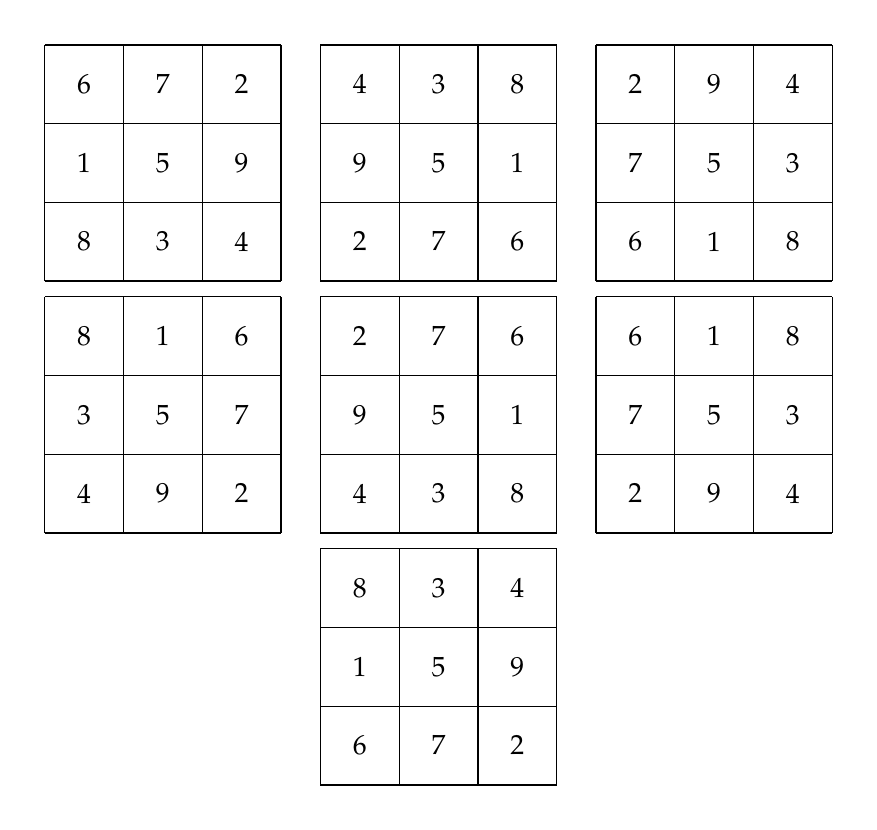
\begin{tikzpicture}[scale=.5]
	    \matrix[row sep=0.cm,column sep=0.3cm] {
		 	\begin{scope}
		 \clip (-0.1,-0.1) rectangle (3.1,3.1);
		 \draw (0, 0) grid (3, 3);
		 \draw[very thin] (0, 0) grid (3, 3);
		 
		 \setcounter{row}{3}
		 \setrow {6}{7}{2}
		 \setrow {1}{5}{9}
		 \setrow {8}{3}{4}
		 \end{scope}
		 	&
		 	\begin{scope}
		 \clip (-0.1,-0.1) rectangle (3.1,3.1);
		 \draw (0, 0) grid (3, 3);
		 \draw[very thin] (0, 0) grid (3, 3);
		 
		 	\setcounter{row}{3}
		 \setrow {4}{3}{8}
		 \setrow {9}{5}{1}
		 \setrow {2}{7}{6}
		 \end{scope}
		 	     &
		 	\begin{scope}
		 \clip (-0.1,-0.1) rectangle (3.1,3.1);
		 \draw (0, 0) grid (3, 3);
		 \draw[very thin] (0, 0) grid (3, 3);
		 
		 \setcounter{row}{3}
			\setrow {2}{9}{4}
		\setrow {7}{5}{3}
		\setrow {6}{1}{8}
		 \end{scope} 
		 		      \\
		 		    	\begin{scope}
		 		    \clip (-0.1,-0.1) rectangle (3.1,3.1);
		 		    \draw (0, 0) grid (3, 3);
		 		    \draw[very thin] (0, 0) grid (3, 3);
		 		    
		 		    \setcounter{row}{3}
		 		    \setrow {8}{1}{6}
		 		    \setrow {3}{5}{7}
		 		    \setrow {4}{9}{2}
		 		    \end{scope}  &
		 		    	\begin{scope}
		 		    \clip (-0.1,-0.1) rectangle (3.1,3.1);
		 		    \draw (0, 0) grid (3, 3);
		 		    \draw[very thin] (0, 0) grid (3, 3);
		 		    
		 		    \setcounter{row}{3}
		 		    \setrow {2}{7}{6}
		 		    \setrow {9}{5}{1}
		 		    \setrow {4}{3}{8}
		 		    \end{scope}
		 		    &
		 		    \begin{scope}
		 		    \clip (-0.1,-0.1) rectangle (3.1,3.1);
		 		    \draw (0, 0) grid (3, 3);
		 		    \draw[very thin] (0, 0) grid (3, 3);
		 		    
		 		    \setcounter{row}{3}
		 		    \setrow {6}{1}{8}
		 		    \setrow {7}{5}{3}
		 		    \setrow {2}{9}{4}
		 		    \end{scope}
		 		    \\
		 		    &
		 		    	\begin{scope}
		 		    \clip (-0.1,-0.1) rectangle (3.1,3.1);
		 		    \draw (0, 0) grid (3, 3);
		 		    \draw[very thin] (0, 0) grid (3, 3);
		 		    
		 		    \setcounter{row}{3}
		 		    \setrow {8}{3}{4}
		 		    \setrow {1}{5}{9}
		 		    \setrow {6}{7}{2}
		 		    \end{scope}
		 		    &\\
		 	};
	\end{tikzpicture}
\end{document}